\section{Previous Work}\label{previous}

\subsection{Industry Standards}
There are several relevant standards that apply to the process model proposed in
this research. While the Software Engineering Institute, the International
Standards Organization, and NASA put forth standards to facilitate the entire
process of software engineering, we are only concerned with the 
\textit{documentation} efforts recommended by these guidelines.

\subsubsection{CMM}
The Cabability Maturity Model, or CMM, is concerned with improving processes.
According to the Software Engineering Institute, the process followed by an
organization exhibits that organization's maturity. The CMM describes:

\begin{quote}\label{process}
``A \textbf{software process} can be defined as a set of activities, methods,
practicies, and transformations that people use to develop and maintain software
and the associated products (e.g., project plans, design documents, code, test
cases, and user manuals).'' \cite{CMM11}
\end{quote}

The techniques laid out by CMM will help undisciplined organizations manage
software projects. By using the infrastructure in the CMM, organizations can 
avoid software projects that finish late or overbudget.

For more information about CMM as it applies to software, please refer to
\cite{CMM11}.

\subsubsection{ISO 9000-3}
The International Standards Organization put forth a quality management standard
known as ISO 9001 to describe a set of guidelines that will help organizations
achieve standards of quality that are recognized and respected throughout the
world. The ISO 9000-3 is the application of ISO 9001 to the field of software
engineering. They describe \textbf{software engineering} as: 

\begin{quote}
``\ldots a defined, step-by-step process that facilitates the specification,
design, implementation, and testing of a software solution for a set of stated
requirements in the most expeditious and cost-effective manner possible.''
\cite{Kehoe1996}
\end{quote}

During this process of software engineering, the ISO 9000-3 standard commands
that software development and maintenance efforts be based upon a defined
process that (among other things): 

\begin{quote}
``\ldots creates \textit{succinct and usable} level of documentation that will
support and facilitate continued enhancements to and maintenance of the product
as well as provide the basis for estimating future efforts.'' \cite{Kehoe1996}
\end{quote}

\subsubsection{NASA-STD-8719.13A}
The National Aeronautics and Space Administration publishes a set of guidelines
and standards that provide a methodology for software safety in their programs.
In \cite{NASA1997} specifically, their organization purposes describe the
activities necessary to ensure that safety is designed into and maintained
throughout the safety critical software lifecycle. NASA describes \textbf{safety
critical software} as software that\ldots

\begin{quote} 
``\ldots exercises direct command and control over the condition or state of
hardware components; and, if not performed, performed out-of-sequence, or
performed incorrectly could result in improper control functions (or lack of
control functions required for proper system operation), which could cause a
hazard or allow a hazardous condition to exist.'' \cite{NASA1997}
\end{quote}

Among other requirements, NASA demands of its software implementations that
safety-critical code ``shall be commented in such a way that future changes can
be made with a reduced likelihood of invoking a hazardous state.''

\subsection{Legal Research}
\begin{figure}
\begin{center}
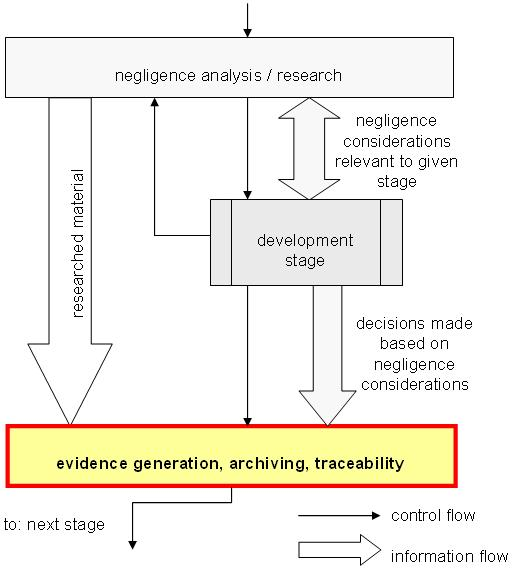
\includegraphics[scale=0.66]{images/enhancement.jpg}
\end{center}
\caption{Enhancement to existing software development stage}
\label{enhancement}
\end{figure}
The legal problems begot by software in safety-critical systems have already
been researched \cite{Turner1996, Turner2000} and some suggestions have been
made to help alleviate the cost of defending the risk associated with
safety-critical systems\cite{Turner2001}. Additionally, it has been identified
that software defects cannot easily be designated as manufacture-defective or
design-defective\cite{Turner2000}, and therefore cannot be classified as
strict-product liable or negligence liable in legal disputes. It is clear that
both aspects of liability be addressed. This research focuses on defects in the
process model vulnerable to negligence allegations.

There has already been work that tries to address this overall problem. Clark
Turner, et. al. has researched the implications of safety-critical systems in
\cite{Turner1996, Turner2000, Turner2001} and as deduced that a popular
approach to this problem is the retroactive investigation of attorneys when a
legal dispute ensues. But this is both inefficient and oftentimes ineffective
because important historical information may be missing and unrecoverable. They
briefly propose an enhanced process model shown in Figure \ref{enhancement} that
will addresses negligence considerations early in the software development
lifecycle \cite{Turner2001}.

\subsection{Documentation Solutions}

In \cite{Parnas1986}, David Parnas encourages documentation to compensate for
rational design. Since it is impossible to build a bug-free system, inadvertent
mistakes are forgivable with requirements and documentation. He lays out
acceptance criteria for ideal requirements documentation that can be applied to
safety-critical software environments. Common approaches include formal
requirement specifications, code comments, or more browseable documents like
Javadoc\cite{Javadoc}.

\subsubsection*{Code Comments}
Code comments are in-line, free-text prose that are embedded in the source code
of a program. Comments are ignored by software compilers and program code with
comments in it would perform identically if the comments were absent. From a
technical standpoint, comments ARE NOT documentation. Comments provide a method
for programmers to write helpful clues for human consumers of the code so that
they can understand it better.

The intent of comments is to allow for better comprehension and maintainabilty
of code when other humans try to read it. Comments have potential to provide
very useful links between developer intent and actual implementation, but suffer
drawbacks. First, comments lie within the code, which arguably obfuscates the
code itself if they are lengthy or used inappropriatly. Comments have no
explicit association to modules, functions, object classes, or packages. There
is no formal way of annotating a plain comment to link it with a specific code
module. Also, comments can only be implicitly associated with a single area
of code. Non-trivial programs are typically modular, and it would be useful to
describe what is being done in a group of related code segments.

\subsubsection*{Javadoc}
Javadoc overcomes some of the drawbacks of normal comments. Javadoc includes a
formal syntax and provides special annotations to do associations with methods,
data members, classes, packages, etc. In addition, Javadoc can be ``compiled''
into a more human-readable HTML document. But Javadoc is considered actual
documentation, which we believe does not belong in the code base itself and
should be separated out for readability and maintainability's sake.
Additionally, Javadoc is also limited by its single-module association and
cannot be linked with multiple areas of code.

\subsection{Documentation Traceability}
There is a need to associate software code with its accompanying documentation.
This documentation includes (but is not limited to) requirements, designs, user
manuals, and other free text documents. Gotel and Finkelstein refer to this as
information-driven traceability wherein practitioners
\begin{quote}
``\ldots link functions, data, requirements and any text in the statement of
requirements that refers to them.'' \cite{Gotel1994}
\end{quote}

This notion of code-to-documentation traceability is motivated by the following
\cite{Antoniol1999}.
\begin{itemize}
  \item Program comprehension
  \item Maintenance
  \item Requirements tracing
  \item Impact analysis
  \item Software reuse
\end{itemize}

Antoniol, et. al. researched information retrieval models to recover 
traceability links between code and free text documentation \cite{Antoniol1999,
Antoniol2000}. Their semi-automated system performs this association with the
underlying assumption that programmers use meaningful names and mnemonics for
identifiers. These mnemonics include method signatures, variable names, and
class definitions. By comparing natural language software documents with source
code identifiers, their system draws associations between documents and
quantifiably scores the accuracy of its matches.

Unfortunately, their solution is crippled by its reliance on programmer
mnemonics. Although identifiers are the only user-defined tokens in source
code, much more semantic information can be drawn from the code itself
beyond mere identifier extraction.


